% !TEX spellcheck = en_US
% !TEX encoding = UTF-8

\documentclass[xcolor={x11names, table}, compress]{beamer}

\usepackage{xcolor}
\usepackage{fontspec}
\usepackage{pgfgantt}
\usepackage{tikz}
\usepackage{amsmath, amssymb, amsfonts}
\usepackage{bm}
\usepackage{eso-pic}
\usepackage{graphicx}
\usepackage{verbatim}
\usepackage{array}
\usepackage{multirow}
\usepackage{eurosym}
\usepackage{makecell}
\usepackage{hhline}
\usepackage[backend=biber]{biblatex}

%   \pgfplotsset{compat=1.15}
\usetikzlibrary{positioning, shapes, calc, arrows}
\hypersetup{pdfstartview={Fit}}

%% Beamer Layout %%%%%%%%%%%%%%%%%%%%%%%%%%%%%%%%%%
\useinnertheme{default}
\usepackage[T1]{fontenc}
\usefonttheme{professionalfonts}

\setbeamerfont{frametitle}{}

\definecolor{BHKpresentationDark}{RGB}{114,133,176}
\definecolor{BHKpresentationDarkGrey}{RGB}{103,116,128}
\definecolor{BHKblue}{RGB}{51,105,153}

\setbeamerfont{title like}{shape=\scshape}
\setbeamercolor*{frametitle}{fg=BHKpresentationDark} 
\setbeamercolor*{lower separation line head}{bg=BHKblue} 
\setbeamercolor*{normal text}{fg=BHKpresentationDarkGrey,bg=white} 
\setbeamercolor*{alerted text}{fg=BHKblue} 
\setbeamercolor*{example text}{fg=black} 
\setbeamercolor*{item}{fg=BHKpresentationDark,bg=gray} 
\setbeamercolor{enumerate item}{fg=BHKpresentationDark}
\setbeamercolor*{structure}{fg=black} 
\setbeamercolor*{palette tertiary}{fg=black,bg=black!10} 
\setbeamercolor*{palette quaternary}{fg=black,bg=black!10} 
\setbeamercovered{transparent}

\setbeamertemplate{navigation symbols}{}
\setbeamertemplate{footline}{%
    \begin{beamercolorbox}[wd=\paperwidth]{footlinecolor}
        
\includegraphics[width=\textwidth]{bar_footline.pdf}
    \end{beamercolorbox}%
}

\setbeamertemplate{frametitle}[default][center]
\setbeamertemplate{caption}[numbered]
\setbeamertemplate{section in toc}[sections numbered]
\setbeamertemplate{subsection in toc}[subsections numbered]

\newcolumntype{P}[1]{>{\raggedright\arraybackslash}p{#1}}

\newcommand{\insertsec}{\thesection.~\insertsection}
\newcommand{\insertsubsec}{\thesection.\thesubsection~\insertsubsection}

\AtBeginSection[]{
\begin{frame}
\vfill
\centering
\begin{beamercolorbox}[sep=8pt,center,shadow=true,rounded=true]{title}
    \usebeamerfont{title}\insertsec\par%
\end{beamercolorbox}
\vfill
\end{frame}
}


%%%%%%%%%%%%%%%%%%%%%%%%%%%%%%%%%%%
%% Start of document %%%%%%%%%%%%%%
%%%%%%%%%%%%%%%%%%%%%%%%%%%%%%%%%%%

\begin{document}
%%%% title slide %%%%%
{\setbeamertemplate{footline}{} 
    \begin{frame}
        \vspace{-1.5cm}
        \hfill\makebox[0.2\paperwidth]{
\includegraphics[width=0.4\textwidth]{logo_wtext}}
        \begin{flushleft}
            \hspace{-1cm}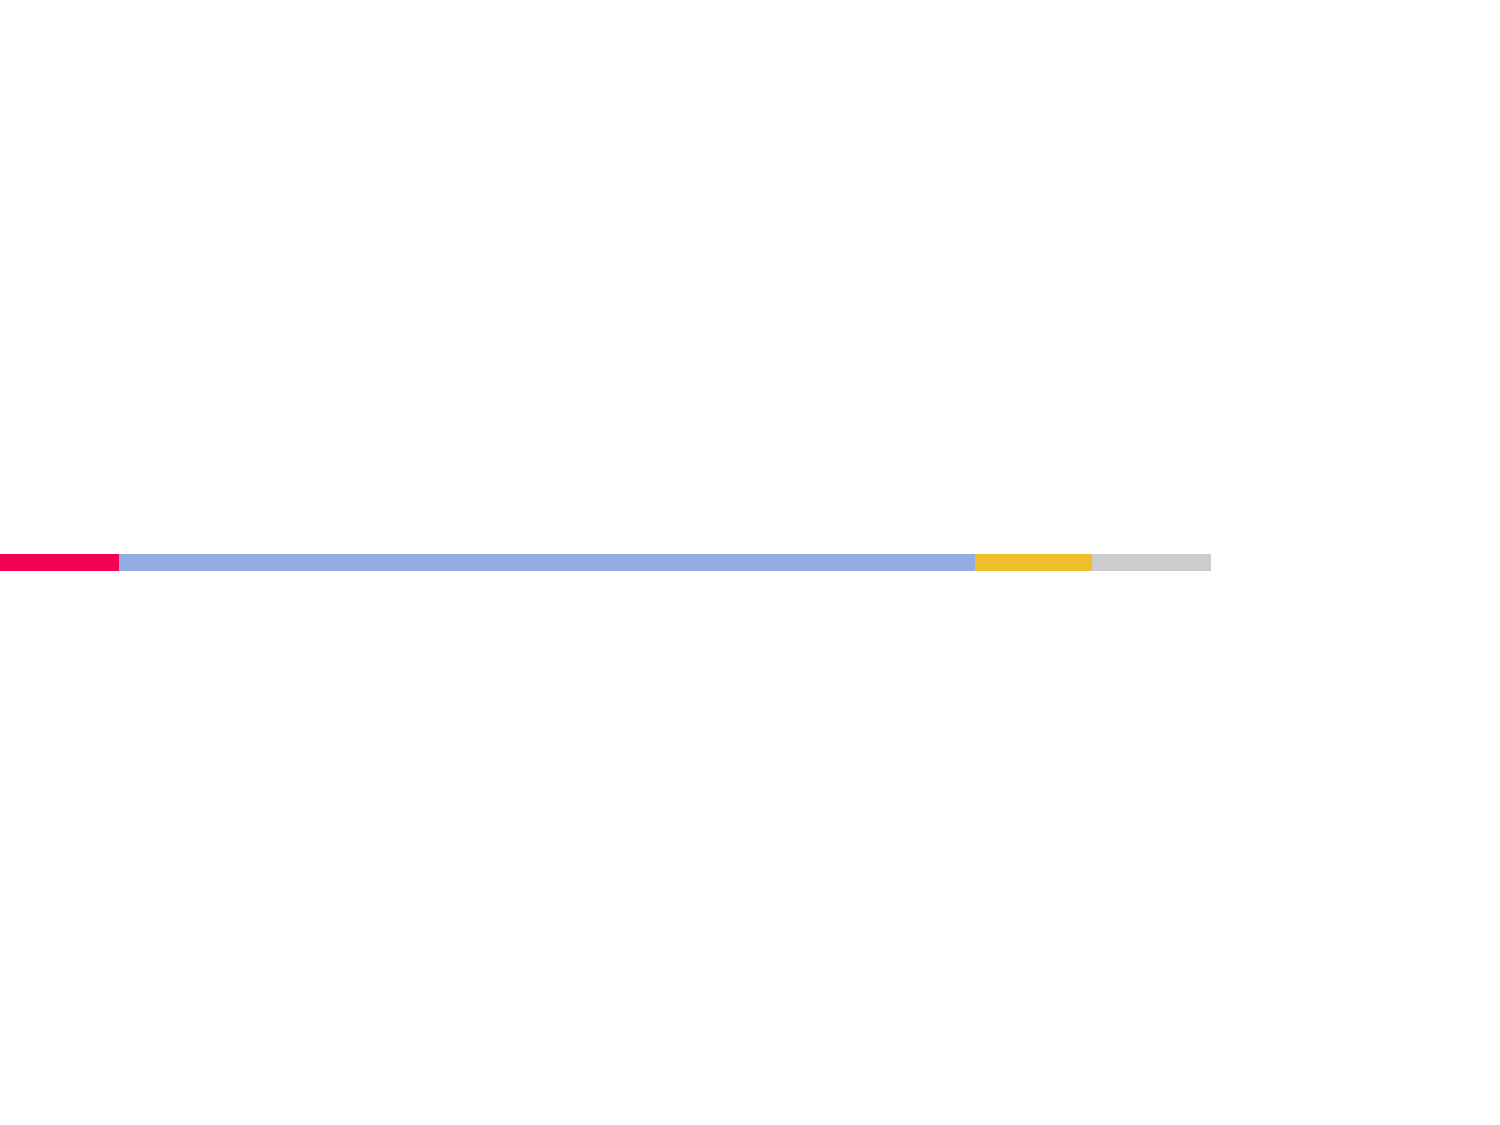
\includegraphics[width=0.8\textwidth, height=0.4em]{title_line.pdf}\hfill
            
            \title{
                \begin{flushleft}{\huge \color{BHKpresentationDark} 
                Unlock the potential of medical imaging using deep learning
            } 
            \end{flushleft}}
            
            \date{$~~$}
            \author[Joan]{\begin{flushleft}\vspace{-1cm} Joan Marcè i Igual\end{flushleft}}
            \titlepage
        \end{flushleft}
    \end{frame}
}

\begin{frame}[allowframebreaks]{Table of Contents}
\tableofcontents[sections={1-3}]
\framebreak
\tableofcontents[sections={4-5}]
\end{frame}

\section{Introduction}
\begin{frame}{\insertsec}
	\begin{itemize}
    \item Nowadays Machine Learning it's widely used
    \item Medical images can be obtained using MRI, PET or CT scans but are underused
    \item Different methods have appeared to analyze these data for image classification,
    object detection, segmentation...
    \item Deep learning models aim to be able to unlock the full potential of medical imaging
  \end{itemize}
\end{frame}

\subsection{Survival Analysis}
\begin{frame}{\insertsubsec}
  Survival analysis models usually have:
  \begin{itemize}
    \item Baseline data \( x \)
    \item Event \( E \in \{0, 1\} \)
    \item Time \( T \)
  \end{itemize}

  Casting the survival problem as a ranking is a way of dealing with censored data.
  \vspace{.3cm}
  \begin{columns}
    \begin{column}{.5\textwidth}
      \begin{figure}
        \centering
        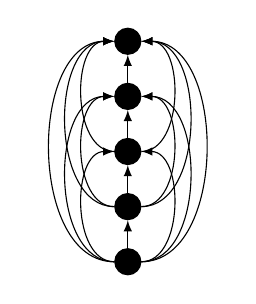
\begin{tikzpicture}[scale=.7]
  \tikzstyle{bDot}=[circle, fill=black, draw]
  \foreach \y in {1,...,5} {
    \node[bDot] (D-\y) at (0, \y) {};
  }

  \foreach \y in {1,...,4} {
    \pgfmathsetmacro{\z}{int(\y + 1)}
    \draw[-latex] (D-\y) -- ({D-\z}.south);
  }

  \foreach \y in {1,...,3} {
    \pgfmathsetmacro{\z}{int(\y + 2)}
    \foreach \j in {\z,...,5} {
      \ifthenelse{\y=2 \OR \y=3}{
        \draw[-latex] (D-\y) to[bend left=90] (D-\j);
      }{
        \draw[-latex] (D-\y) to[bend right=90] (D-\j);
      }
    }
  }
\end{tikzpicture}

        \caption{Uncensored data}
      \end{figure}
    \end{column}
    \begin{column}{.5\textwidth}
      \begin{figure}
        \centering
        \begin{tikzpicture}
  \foreach \y in {1,...,5} {
    \ifthenelse{\y=2 \OR \y=4}{
      \node [circle, fill=white, draw=black] (D-\y) at (0, \y) {};
    }{
      \node [circle, fill=black, draw=black] (D-\y) at (0, \y) {};
    }

    \foreach \y in {3,4,5} {
      \draw [-latex] (D-1) to[bend right=90] (D-\y);
    }

    \foreach \y/\z in {1/2, 3/4} {
      \draw [-latex] (D-\y) -- (D-\z);
    }
    \draw [-latex] (D-3) to[bend left=90] (D-5);
  }
\end{tikzpicture}

        \caption{Censored data}
      \end{figure}
    \end{column}
  \end{columns}
  
\end{frame} 
\section{Context}
\subsection{Problem formulation}
\begin{frame}{\insertsubsec}
  \begin{itemize}
    \item We have access to a unique set of \( \simeq 500 \) scans
    \item Develop a new deep learning model to analyze this dataset
    \item Get better results than the \emph{volume} radiomic feature which usually achieves
    a C-index of 0.65 for the Head and Neck dataset. 
  \end{itemize}
\end{frame}

\subsection{State-of-the-art}
\begin{frame}{\insertsubsec}
  The most typical approach is to extract radiomic features, usually with
  the \emph{PyRadiomics} package, from the MRI, PET or CT scans.

  \vspace{.5cm}
  An alternative approach is to use deep-learning based models for prediction or 
  feature extraction. Pre-trained models have reduced the requirements for big data sets.
  Possible strategies are:
  \begin{itemize}
    \item Use a pre-trained CNN as a feature extractor
    \item Fine tune a pre-trained CNN on medical data
  \end{itemize}
  
\end{frame}

\subsection{Stakeholders}
\begin{frame}{\insertsubsec}
  \begin{itemize}
    \item Developer: responsible for research, document and implement the software
    \item Director: responsible for guiding, giving advice and helping the Developer
    \item Beneficiaries: future researchers or patients depending on the outcome
  \end{itemize}
\end{frame}

\subsection{Methodology}
\begin{frame}{\insertsubsec}
  \begin{itemize}
    \item As a research project it will have a process of trial and error
    \item Once in a while the project will be presented in the lab weekly meetings
    \item Every week a meeting with the Principal Investigator will be scheduled
  \end{itemize}
\end{frame}

\subsection{Obstacles}
\begin{frame}{\insertsubsec}
  Some obstacles may be found during the project:

  \begin{itemize}
    \item Training time
    \item Bugs
    \item Scheduling
    \item Not enough data
  \end{itemize}
\end{frame}

\section{Planning}
\subsection{Tasks}
\subsection{Estimated time}
\subsection{Alternatives}
\section{Budget}
\subsection{Hardware}
\begin{frame}{\insertsubsec}
  \begin{table}[H]
    \centering
    \footnotesize
    \begin{tabular}{|p{3cm}|r|r|r|r|}
      \hline
      \textbf{Product} & \textbf{Price (\euro)} & \textbf{Units} & \textbf{Useful life} 
      & \textbf{Amortization (\euro)} \\ \hline\hline
  
      MSI GL62M 7RD-429XES & 1.000 \euro & 1 & 5 years & 83 \euro \\ \hline
      Lab iMac & 0 \euro & 1 & -- & 0 \euro \\ \hline
      Compute Canada platform & 0 \euro & 1 & -- & 0 \euro \\ \hline
  
      \hline\hline
      \textbf{Total} & 1.000 \euro & \multicolumn{2}{|c|}{} & 83 \euro \\ \hline
    \end{tabular}
    \caption{Hardware budget \label{tab:hardware-budget}}
  \end{table}
\end{frame}

\subsection{Software}
\begin{frame}{\insertsubsec}
  \begin{table}[H]
    \centering
    \begin{tabular}{|l|r|r|r|}
      \hline
      \textbf{Product} & \textbf{Price} & \textbf{Units} & \textbf{Amortization} \\ \hline\hline
  
      Python & 0 \euro & 1 & 0 \euro \\ \hline
      Tensorflow & 0 \euro & 1 & 0 \euro \\ \hline
      PyDicom & 0 \euro & 1 & 0 \euro \\ \hline
      NumPy & 0 \euro & 1 & 0 \euro \\ \hline
      Scikit & 0 \euro & 1 & 0 \euro \\ \hline
      Visual Studio Code & 0 \euro & 1 & 0 \euro \\ \hline
      Git & 0 \euro & 1 & 0 \euro \\ \hline
      GitHub & 0 \euro & 1 & 0 \euro \\ \hline
      PyCharm Community Edition & 0 \euro & 1 & 0 \euro \\ \hline
      \LaTeX & 0 \euro & 1 & 0 \euro \\ \hline
      Vim & 0 \euro & 1 & 0 \euro \\ \hline
  
      \hline\hline
      \textbf{Total} & 0 \euro &  & 0  \euro \\ \hline
    \end{tabular}
    \caption{Software budget \label{tab:software-budget}}
  \end{table}
\end{frame}

\subsection{Human resources}
\begin{frame}[allowframebreaks]{\insertsubsec}
  \begin{table}[H]
    \centering
    \begin{tabular}{|l|r|r|r|}
      \hline
      \textbf{Role} & \textbf{Hours} & \textbf{\euro/hour} & \textbf{Salary} \\ \hline\hline
  
      Project Manager & 70 & 26 & 1.820 \euro \\ \hline
      Software Developer & 510 & 18 & 9.180 \euro \\ \hline
      Tester & 180 & 15 & 2.700 \euro \\ \hline
  
      \hline\hline 
      Total & 760 & & 13.700 \euro \\
      \hline
    \end{tabular}
  
    \caption{Human resources budget \label{tab:salary}}
  \end{table}
  \framebreak
  \footnotesize
  \begin{table}[H]
    \centering
    \begin{tabular}{|P{3cm}|r|r|r|r|}
      \hline
      \multirow{2}{*}[-1em]{\textbf{Task}} & 
      \multirow{2}{*}[-1em]{\textbf{Duration}} & 
      \multicolumn{3}{|c|}{\textbf{Dedication}} \\ \cline{3-5}
  
       & & \parbox[c][1.5cm]{1.6cm}{\textbf{Project \\ Manager}} & 
       \parbox[c][1.5cm]{1.6cm}{\textbf{Software \\ Developer}} & 
       \textbf{Tester} \\ \hline\hline
  
       Acquire background in CNN & 120 & 10 & 110 & 0 \\ \hline
       Get familiar with survival models & 80 & 10 & 70 & 0 \\ \hline
       Preprocess data & 40 & 10 & 20 & 10 \\ \hline
       Build shallow siamese network & 200 & 15 & 110 & 75 \\ \hline
       Build deep siamese network & 80 & 10 & 50 & 20 \\ \hline
       Compare models & 80 & 10 & 40 & 30 \\ \hline
       Final stage & 160 & 5 & 110 & 45 \\ 
  
       \hline\hline
       \textbf{Total} & 760 & 70 & 510 & 180 \\
       \hline
    \end{tabular}
  
    \caption{Time estimation by role \label{tab:time-estimation}}
  \end{table}
\end{frame}

\subsection{Unexpected costs}
\begin{frame}{\insertsubsec}
  \begin{table}[H]
    \centering
    \begin{tabular}{|l|r|r|r|}
      \hline
      \textbf{Role} & \textbf{Hours} & \textbf{\euro / hour} & \textbf{Salary} \\ \hline\hline
      Project Manager & 10 & 26 & 260 \euro \\ \hline
      Software Developer & 20 & 18 & 360 \euro \\ \hline
      Tester & 10 & 15 & 150 \euro \\ \hline
  
      \hline\hline
      \textbf{Total} & 40 & & 770 \euro \\ 
      \hline
    \end{tabular}
    \caption{Unexpected costs \label{tab:unexpected-costs}}
  \end{table}
\end{frame}

\subsection{Indirect costs}
\begin{frame}{\insertsubsec}
  \begin{table}[H]
    \centering
    \begin{tabular}{|l|r|r|r|}
      \hline
      \textbf{Product} & \textbf{Price} & \textbf{Units} & \textbf{Cost} \\ \hline\hline
  
      Electricity & 0,12 \euro/kWh & 550 kWh & 66 \euro \\ \hline
      Internet + phone & 70 \euro/month & 4 months & 280 \euro \\ \hline
      
      \hline\hline
      \textbf{Total} & & & 346 \euro \\ \hline
    \end{tabular}
    \caption{Indirect costs \label{tab:indirect-costs}}
  \end{table}
\end{frame}

\subsection{Total budget}
\begin{frame}{\insertsubsec}
  \begin{table}[H]
    \centering
    \begin{tabular}{|l|r|}
      \hline
      \textbf{Concept} & \textbf{Estimated Costs} \\ \hline\hline
  
      Hardware resources & 83 \euro \\ \hline
      Software resources & 0 \euro \\ \hline
      Human resources & 13.700 \euro \\ \hline
      Unexpected costs & 770 \euro \\ \hline
      Indirect costs & 346 \euro \\ \hline
  
      \hline\hline
      \textbf{Subtotal} & 14.899 \euro \\
      \hline\hline
      Contingency (5\%) & 744.95 \euro \\
      \hline\hline
      \textbf{Total} & \textbf{15.643,95 \euro} \\ \hline
    \end{tabular}
  
    \caption{Total project costs \label{tab:total-costs}}
  \end{table}
\end{frame}


\section{Sustainability}
\subsection{Environmental}
\subsection{Social}
\subsection{Economical}


\begin{frame}
    \begin{center}
        Questions?
    \end{center}
\end{frame}



\end{document}